\documentclass[accentcolor=tud4b,colorbacktitle,inverttitle,landscape,german,presentation,t]{tudbeamer}
\mathcode`\,="013B%L�scht das Leerzeichen nach dem Komma in Dezimalzahlen
%\usepackage{multimedia}

%\usepackage{media9}

%\usepackage{movie15}


\usepackage{hyperref}
\usepackage{bbding}
\usepackage{units}
\usepackage{epstopdf}
\usepackage{subfigure}
\usepackage{caption}
\usepackage{ngerman}
\usepackage{color}
\usepackage{rotating}
%\usepackage[latin1]{inputenc}   % deutsche Umlaute
\usepackage[T1]{fontenc}        % Darstellung von Schrift als echte T1 Fonts und nicht als Bilder
\usepackage{graphicx}
\input{header}

%
% Macros
%
% \renewcommand{\vec}[1]{\ensuremath{\bm{#1}}}
\renewcommand{\vec}[1]{\ensuremath{\boldsymbol{#1}}}

\begin{document}
\title[]{Survey on Image Classification in the Domain Mixture Scenario}
\subtitle{Bachelor Thesis}
\author[Runchida Kaewngoen]{Runchida Kaewngoen}
\institute[Regelungsmethoden und Robotik | Bachelor Thesis]{Regelungsmethoden und Robotik | Bachelor Thesis}




% \logo{\color{tudtextaccent}TU Darmstadt-}
\logo{\includegraphics{rmr2}}

\date{26.02.2020}	
%Titelfolie%%%%%%%%%%%%%%%%%%%%%%%%%%%%%%%%%%%%%%%%%%%%%%%%%%%%%%%%%%%%%%%%%%%%%%%%%%%%%%%%%%%%%%%%%%%%%%%%%%%%%%%%%%%%%%%%%%%%%%%%%%%%%%%%%%%%%%%%%%%%%%%%%%%
\begin{titleframe}
	\begin{center}
	\vspace{3cm}
		\begin{figure}
		\includegraphics[width=0.8\linewidth]{bilder/IntroPic.png}
		\end{figure} 
	\end{center}
\end{titleframe}

%Hauptfolien%%%%%%%%%%%%%%%%%%%%%%%%%%%%%%%%%%%%%%%%%%%%%%%%%%%%%%%%%%%%%%%%%%%%%%%%%%%%%%%%%%%%%%%%%%%%%%%%%%%%%%%%%%%%%%%%%%%%%%%%%%%%%%%%%%%%%%%%%%%%%%%%%%%
%%%%%%%%%%

\begin{frame}{\\Motivation}
	\vspace{-0.5cm}
	\begin{figure}
		\centering
		\includegraphics[width=\linewidth]{bilder/Motivation.png}
	\end{figure}
\end{frame}

\begin{frame}{\\Overview}
 	\begin{itemize}
  		\item Domain Adaptation
 		\item Domain Mixture Scenario [1]
		\item Domain Separation Networks (DSN) [2]
 		\item Experimental Setups
		\item Results
		\item Conclusion
	\end{itemize}
\end{frame}

\begin{frame}{\\Definitions}
	\visible<2->{\structure{Domain $\mathcal{D}_S$:} A data space with an underlying data distribution. \\ }  \vspace{0.1cm}
	\visible<3->{\structure{Source Domain $\mathcal{D}_S$:} A domain on which the system is trained on. \\ }  \vspace{0.1cm}
	\visible<4->{\structure{Target Domain $\mathcal{D}_T$:} A domain on which the system should perform the task.\\ \vspace{0.2cm}}
	\visible<5->{
		\begin{figure}
			\centering
			\includegraphics[width=0.8\linewidth]{bilder/Domains.png}
		\end{figure}
	}
\end{frame}

\begin{frame}{\\Domain Adaptation}
	\begin{center}
		\visible<1->{
  			\begin{figure}
			\centering
			\includegraphics[width=0.7\linewidth]{bilder/domainAdaptation.jpg}
			\end{figure} 
		} \vspace{0.2cm}
		\visible<2->{\large Goal: Performing well on both domains} \\ \vspace{0.2cm}
	\end{center}
\end{frame}

\begin{frame}{\\Scenarios of Domain Adaptation \tiny [1]}
	\begin{center}
		\begin{figure}
			\centering
			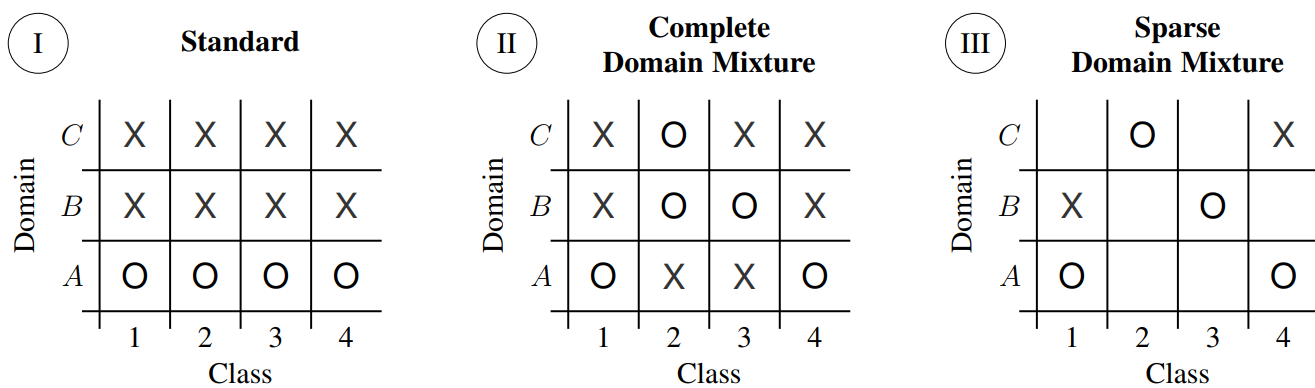
\includegraphics[width=\linewidth]{bilder/scenarioDA.png}
		\end{figure} \vspace{0.5cm}
		O = supervised\\X = unsupervised 
		\tiny [1]
	\end{center}
\end{frame}

\begin{frame}{\\Complete Domain Mixture Scenario\tiny [1]}
	\begin{center}
		\begin{figure}
			%grünes häkchen in den Bildern
			\centering
			\includegraphics[width=\linewidth]{bilder/DomainMixtureExC.png}
		\end{figure} \vspace{0.5cm}
		O = supervised\\X = unsupervised 
	\end{center}
\end{frame}

\begin{frame}{\\Domain Separation Networks (DSN) \tiny [2]}
	\begin{center}
		\only<1-2>{\begin{figure}
			\centering
			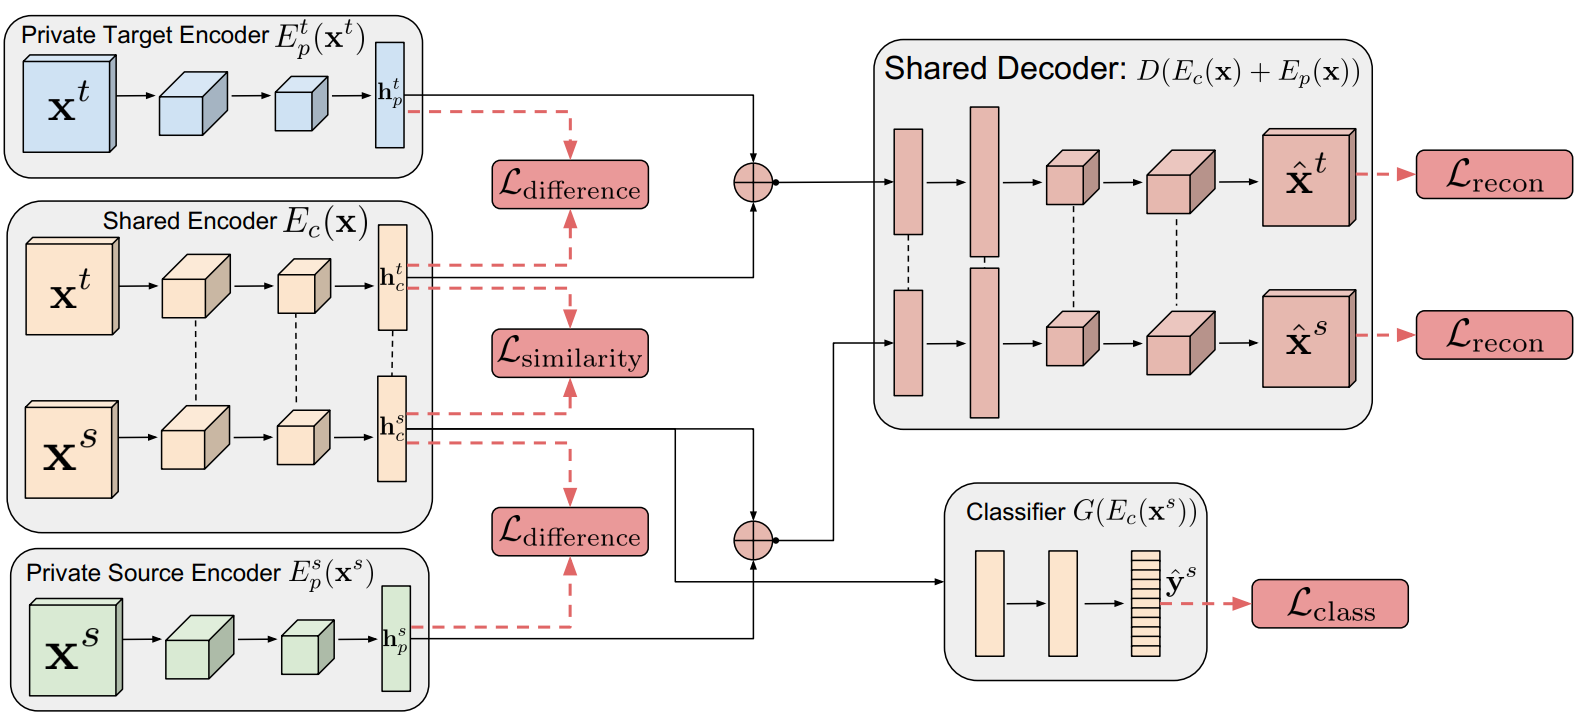
\includegraphics[width=0.8\linewidth]{bilder/DSN.png}
			\end{figure}  
		} 
		\only<3>{\begin{figure}
			\centering
			\includegraphics[width=0.8\linewidth]{bilder/DSNclassi.png}
			\end{figure} 
		} 
		\only<4>{\begin{figure}
			\centering
			\includegraphics[width=0.8\linewidth]{bilder/DSNshared.png}
			\end{figure} 
		} 
		\only<5>{\begin{figure}
			\centering
			\includegraphics[width=0.8\linewidth]{bilder/DSNprivate.png}
			\end{figure} 
		} 
		\only<6>{\begin{figure}
			\centering
			\includegraphics[width=0.8\linewidth]{bilder/DSNdecoder.png}
			\end{figure} 
		} 

		\vspace{0.2cm}
 		\visible<2->{DSN = } \visible<3->{Classifier + } \visible<4->{Shared Encoder + } \visible<5->{Private Encoders + } \visible<6->{Decoder}
	\end{center}
\end{frame}

\begin{frame}{\\DSN: Loss Functions}
	\begin{center}
		\visible<1->{
			$\mathcal{L} = \mathcal{L}_{Task} + \alpha \mathcal{L}_{recon} + \beta \mathcal{L}_{difference} + \gamma \mathcal{L}_{similarity}$ \\ \vspace{0.2cm}
		}
	\end{center}
	\only<1>{\begin{figure}
			\centering
			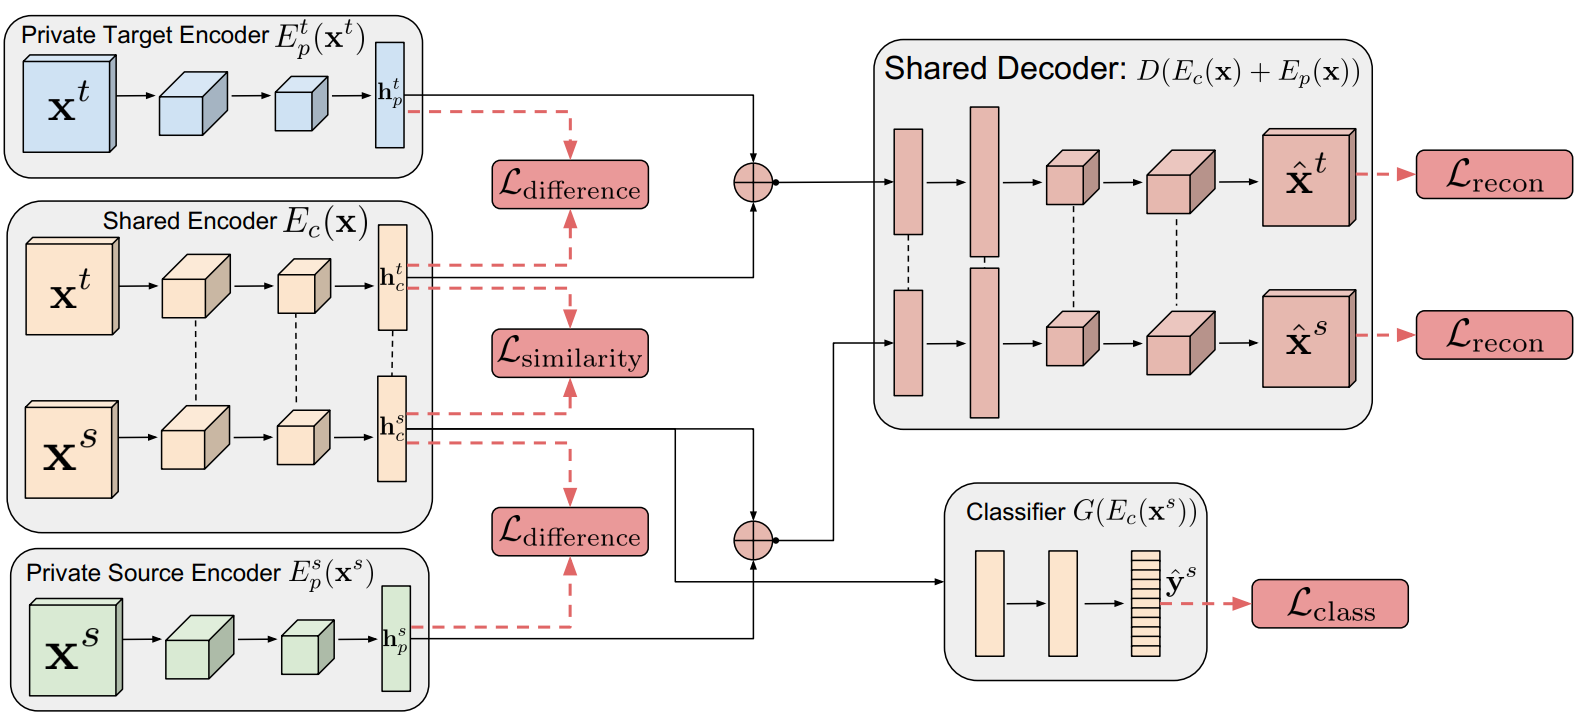
\includegraphics[width=0.8\linewidth]{bilder/DSN.png}
			\end{figure}  
	} 
	\only<2>{\begin{figure}
			\centering
			\includegraphics[width=0.8\linewidth]{bilder/DSNLtask.png}
			\end{figure}  
	} 
	\only<3>{\begin{figure}
		\centering
		\includegraphics[width=0.8\linewidth]{bilder/DSNLrecon.png}
		\end{figure} 
	} 
	\only<4>{\begin{figure}
		\centering
		\includegraphics[width=0.8\linewidth]{bilder/DSNLdiff.png}
		\end{figure} 
	} 
	\only<5>{\begin{figure}
		\centering
		\includegraphics[width=0.8\linewidth]{bilder/DSNLsim.png}
		\end{figure} 
	} 
\end{frame}

\begin{frame}{\\Datasets}
	\begin{center}
	\vspace{1cm}
		\begin{figure}
			\centering
			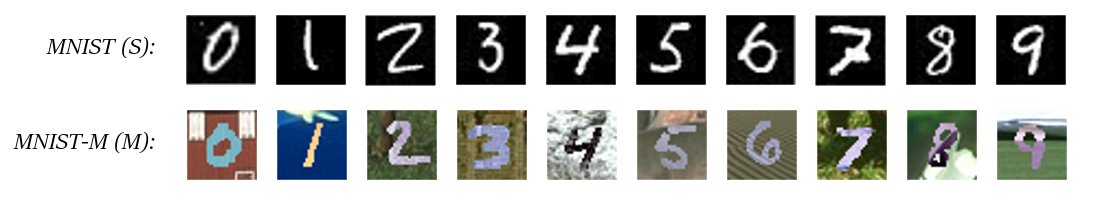
\includegraphics[width=\linewidth]{bilder/mnistmnistmText.png}
			\end{figure} 
	\end{center}
\end{frame}

\begin{frame}{\\Experimental Setups}
	\visible<1->{ \begin{block}{Objectives:} \end{block}
		Investigating the Complete Domain Mixture Scenario using DSN with different loss combinations}
	\vspace{0.5cm}
	\visible<2->{ \begin{block}{Procedures:}\end{block} \vspace{-0.5cm}
	\begin{itemize}
		\item Different mixtures in the Complete Domain Mixture Scenario
		\item Different loss combinations of the DSN
		\item Each cases 10 runs}
	\end{itemize}
\end{frame}

\begin{frame}{\\Experimental Setups: Example}
	\begin{center}
	\begin{figure}
		\centering
		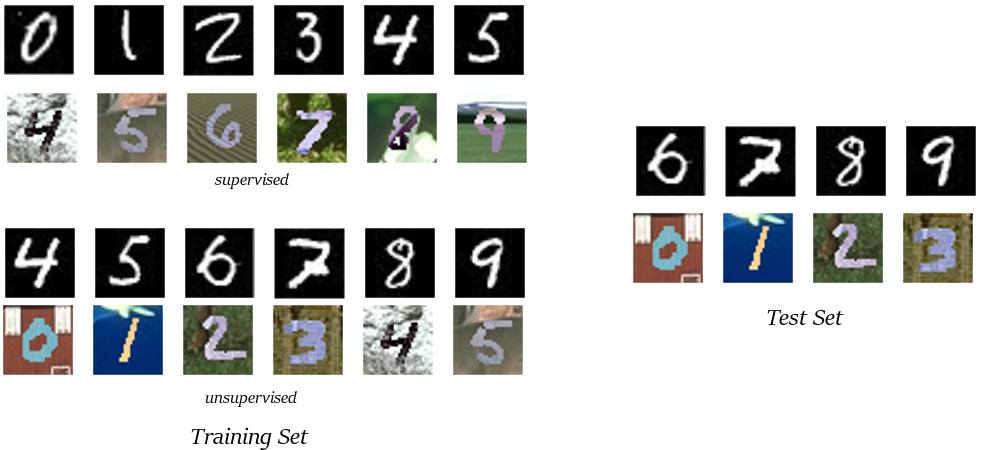
\includegraphics[width=\linewidth]{bilder/mixeddomain.png}
	\end{figure}
	Number of supervised class $m = 6$ 
	\end{center}
\end{frame}

\begin{frame}{\\Experimental Setups}
	\begin{center}
		$\mathcal{L} = \mathcal{L}_{Task} + \alpha \mathcal{L}_{recon} + \beta \mathcal{L}_{difference} + \gamma \mathcal{L}_{similarity}$ \\ \vspace{1cm}
		\begin{itemize}
		\item<2-> DSN = all losses activated
		\item<3-> noDA = no domain adaptation = no loss activated
		\item<4-> sim = only $\mathcal{L}_{similarity}$ activated
		\item<5-> nosim = only $\mathcal{L}_{similarity}$ deactivated
		\item<6-> $\cdots$
		\end{itemize}
		
	\end{center}
\end{frame}

\begin{frame}{\\Results}
	\vspace{-0.6cm}
	\begin{figure}
		\centering
		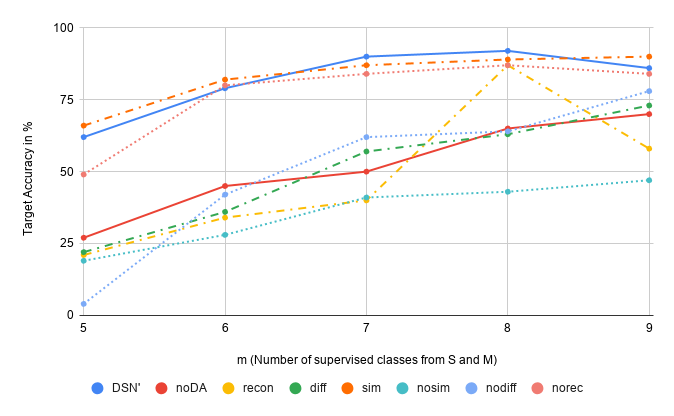
\includegraphics[width=0.9\linewidth]{bilder/allDSNResults.png}
	\end{figure}
\end{frame}

\begin{frame}{\\Open Questions}
	\begin{itemize}
		\item<2-> Relatively big performance gap between $m = 5$ and $m = 6$
		\item<3-> Radical bad results in some runs within the same setup
	\end{itemize}
\end{frame}

\begin{frame}{\\Conclusion}
	\begin{center}
	\begin{figure}
		\centering
		\includegraphics[width=0.8\linewidth]{bilder/DMrobot.png}
	\end{figure}
	\tiny [1]
	\end{center}
\end{frame}

\begin{frame}{\\Sources}
	[1] Schrom, Sebastian ; Hasler, Stephan: Domain Mixture: An Overlooked Scenario in Domain Adaptation, 2019 \\ \vspace{0.2cm}
	{[2]} Bousmalis, Konstantinos ; Trigeorgis, George ; Silberman, Nathan ; Krishnan, Dilip ; Erhan, Dumitru: Domain Separation Networks. In: CoRR abs/1608.06019 (2016). http://arxiv.org/abs/1608.06019 \\ \vspace{0.2cm}
	{[3]} Ganin, Yaroslav ; Ustinova, Evgeniya ; Ajakan, Hana ; Germain, Pascal ; Larochelle, Hugo; Laviolette, François ; Marchand, Mario ; Lempitsky, Victor S.: Domain-Adversarial Training of Neural Networks. In: J. Mach. Learn. Res. 17 (2015), S. 59:1–59:35 \\\vspace{0.2cm}
	{[4]} Ding, Z. ; Shao, M. ; Fu, Y.: Incomplete Multisource Transfer Learning. In: IEEE Transactions on Neural Networks and Learning Systems 29 (2018), Feb, Nr. 2, S. 310–323. http://dx.doi.org/10.1109/TNNLS.2016.2618765. – DOI 10.1109/TNNLS.2016.2618765. – ISSN 2162–2388	\vspace{0.2cm}
\end{frame}

\end{document}
